% JADE Metrics data flow diagram
% Template adapted from http://www.texample.net/tikz/examples/data-flow-diagram/ by David Fokkema
\documentclass{article}
\usepackage{tikz}
\usetikzlibrary{arrows,shapes}

% Custom, should be provided in the same directory.
\usepackage{datastore}

% Disable page number for better SVG.
\pagenumbering{gobble}

\begin{document}
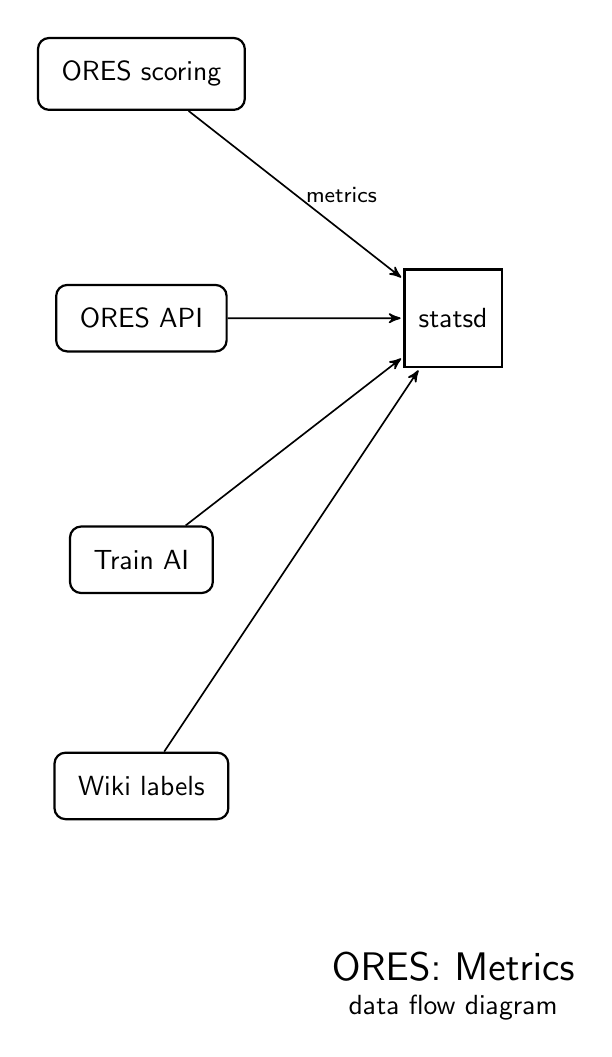
\begin{tikzpicture}[
  font=\sffamily,
  every matrix/.style={ampersand replacement=\&,column sep=2cm,row sep=2cm},
  interface/.style={draw,thick,regular polygon,regular polygon sides=4,inner sep=0},
  process/.style={draw,thick,rounded corners,inner sep=.3 cm},
  datastore/.style={draw,thick,shape=datastore,inner sep=.3cm},
  to/.style={->,>=stealth',shorten >=1pt,semithick,font=\sffamily\footnotesize},
  every node/.style={align=center}]

  % Position the nodes using a matrix layout
  \matrix{
    \node[process] (scoring) {ORES scoring}; \\
    \node[process] (api) {ORES API};
      \& \node[interface] (statsd) {statsd}; \\
    \node[process] (train) {Train AI}; \\
    \node[process] (wikilabels) {Wiki labels};
      \& \node (hidden) {}; \\
  };

  \node [below=2cm, align=flush center] at (hidden)
  {\Large ORES: Metrics \\ \normalsize data flow diagram};

  % Draw and label arrows between nodes.
  \draw[to] (scoring) -- node[midway,right] {metrics} (statsd);
  \draw[to] (api) -- node[midway,above] {} (statsd);
  \draw[to] (train) -- node[midway,above] {} (statsd);
  \draw[to] (wikilabels) -- node[midway,above] {} (statsd);
\end{tikzpicture}
\end{document}
